Download

Source

PDF
Actions
   Copy Project
   Word Count
Sync
   Dropbox
   Git
   GitHub
Settings
Compiler

pdfLaTeX
TeX Live version

2016 (Overleaf v1) (Legacy)
Main document

sample.tex
Spell check

Spanish
Auto-complete

On
Auto-close Brackets

On
Code check

On
Editor theme

overleaf
Overall theme

Default
Keybindings

None
Font Size

12px
Font Family

Lucida / Source Code Pro
Line Height

Normal
PDF Viewer

Built-In
Help
   Show Hotkeys
   Documentation
   Contact Us
Back to your projects
Protocolo Seminario de proyectos

File outline
 Imported from Another project/Diagramas/virus.tex, at 1:30 pm Tue, 17th Aug 21

 


\tikzset{every picture/.style={line width=0.75pt}} %set default line width to 0.75pt        

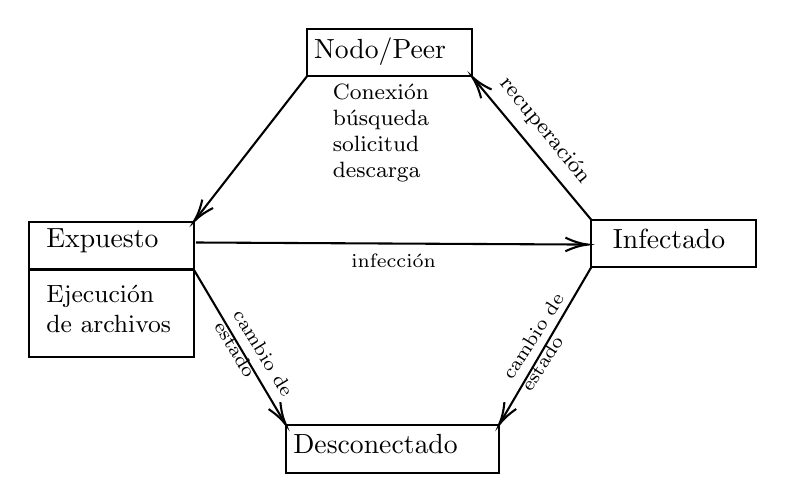
\begin{tikzpicture}[x=0.75pt,y=0.75pt,yscale=-1,xscale=1]
%uncomment if require: \path (0,300); %set diagram left start at 0, and has height of 300

%Shape: Rectangle [id:dp8892068826347792] 
\draw   (260,55) -- (339.5,55) -- (339.5,78) -- (260,78) -- cycle ;
%Shape: Rectangle [id:dp3251536718800727] 
\draw   (126,148) -- (205.5,148) -- (205.5,171) -- (126,171) -- cycle ;
%Shape: Rectangle [id:dp5581801427400581] 
\draw   (397,147) -- (476.5,147) -- (476.5,170) -- (397,170) -- cycle ;
%Shape: Rectangle [id:dp20729403833446924] 
\draw   (250,246) -- (352.5,246) -- (352.5,269) -- (250,269) -- cycle ;
%Straight Lines [id:da4909754265155548] 
\draw    (260,78) -- (206.73,146.42) ;
\draw [shift={(205.5,148)}, rotate = 307.9] [color={rgb, 255:red, 0; green, 0; blue, 0 }  ][line width=0.75]    (10.93,-3.29) .. controls (6.95,-1.4) and (3.31,-0.3) .. (0,0) .. controls (3.31,0.3) and (6.95,1.4) .. (10.93,3.29)   ;
%Straight Lines [id:da719599505686886] 
\draw    (206.5,158) -- (393.5,158.99) ;
\draw [shift={(395.5,159)}, rotate = 180.3] [color={rgb, 255:red, 0; green, 0; blue, 0 }  ][line width=0.75]    (10.93,-3.29) .. controls (6.95,-1.4) and (3.31,-0.3) .. (0,0) .. controls (3.31,0.3) and (6.95,1.4) .. (10.93,3.29)   ;
%Straight Lines [id:da7436102667551165] 
\draw    (397,170) -- (353.51,244.27) ;
\draw [shift={(352.5,246)}, rotate = 300.35] [color={rgb, 255:red, 0; green, 0; blue, 0 }  ][line width=0.75]    (10.93,-3.29) .. controls (6.95,-1.4) and (3.31,-0.3) .. (0,0) .. controls (3.31,0.3) and (6.95,1.4) .. (10.93,3.29)   ;
%Straight Lines [id:da8219422282271829] 
\draw    (397,147) -- (340.78,79.54) ;
\draw [shift={(339.5,78)}, rotate = 410.19] [color={rgb, 255:red, 0; green, 0; blue, 0 }  ][line width=0.75]    (10.93,-3.29) .. controls (6.95,-1.4) and (3.31,-0.3) .. (0,0) .. controls (3.31,0.3) and (6.95,1.4) .. (10.93,3.29)   ;
%Straight Lines [id:da2418615733833709] 
\draw    (205.5,171) -- (248.98,244.28) ;
\draw [shift={(250,246)}, rotate = 239.32] [color={rgb, 255:red, 0; green, 0; blue, 0 }  ][line width=0.75]    (10.93,-3.29) .. controls (6.95,-1.4) and (3.31,-0.3) .. (0,0) .. controls (3.31,0.3) and (6.95,1.4) .. (10.93,3.29)   ;
%Shape: Rectangle [id:dp3895878987821779] 
\draw   (126,171) -- (205.5,171) -- (205.5,213) -- (126,213) -- cycle ;

% Text Node
\draw (133,150) node [anchor=north west][inner sep=0.75pt]   [align=left] {Expuesto};
% Text Node
\draw (252,249) node [anchor=north west][inner sep=0.75pt]   [align=left] {Desconectado};
% Text Node
\draw (262,58) node [anchor=north west][inner sep=0.75pt]   [align=left] {Nodo/Peer};
% Text Node
\draw (406,150) node [anchor=north west][inner sep=0.75pt]   [align=left] {Infectado};
% Text Node
\draw (133,177) node [anchor=north west][inner sep=0.75pt]  [font=\small] [align=left] {Ejecución\\de archivos};
% Text Node
\draw (358.56,74.78) node [anchor=north west][inner sep=0.75pt]  [font=\footnotesize,rotate=-50.52] [align=left] {recuperación};
% Text Node
\draw (271,80) node [anchor=north west][inner sep=0.75pt]  [font=\footnotesize] [align=left] {Conexión\\búsqueda\\solicitud\\descarga};
% Text Node
\draw (280,162) node [anchor=north west][inner sep=0.75pt]  [font=\scriptsize] [align=left] {infección};
% Text Node
\draw (351.41,221.58) node [anchor=north west][inner sep=0.75pt]  [font=\scriptsize,rotate=-302.64] [align=left] {cambio de\\estado};
% Text Node
\draw (230.18,187.41) node [anchor=north west][inner sep=0.75pt]  [font=\scriptsize,rotate=-58.53] [align=left] {cambio de\\estado};


\end{tikzpicture}

